\label{sec:core-results}

\subsection{Reliability map}

The qualification account below summarizes the current evidence for all seven
candidate markers. Grade (1) and phenotype (2) reach the strongest tier, \emph{externally
transportable}: NADT-fitted probes, applied with no retraining, reproduce their association in
PANDA (marker 1: $\rho=+0.40$; marker 2: AUROC$=0.82$, both institutions) and, for marker 1, in
PRECISE against real pathologist Gleason score ($\rho=+0.87$, $n=17$, Figure~\ref{fig:m1ext}a).
PTEN loss (4) is multisite-stable within TCGA-PRAD across six tissue-source sites
(leave-one-site-out AUROC $0.59$--$0.69$), but its nested grade-adjusted increment is uncertain
as shown in Section~\ref{sec:confounder-audits}; this is not an independent-cohort validation.
ERG (3) is \emph{internally supported, externally untested}: no independent cohort with
ERG-stained images and Gleason score exists (confirmed by an exhaustive dataset search), but
the association reproduces, and is in fact stronger, with a second encoder (Virchow
$\rho=+0.66$ vs.\ CONCH $\rho=+0.52$--$0.59$). In the completed Gate A grid, AR activity
(6) is positive in all 60 cells ($\rho=0.136$--$0.297$): its positive pooled direction is
consistent across the correlated Gate A settings. Site heterogeneity and transportability are
neither supported nor refuted, its grade-independent increment remains unresolved, and no
scanner, stain, or site causality is inferred. R5 adds six-site patient descriptors and
page-0 metadata, but all six leave-one-site-out intervals include zero and scanner/stain remain
inseparable from site; C05 evidence closure is complete while transportability remains
unresolved. SPOP
mutation (5) is unsupported in the frozen primary configuration and configuration-sensitive
in Gate A (AUROC 0.348--0.679; 25/60 chance-or-worse cells). Thus neither a robust positive nor
a robust null is established; a modest effect and tumor dilution remain unresolved. C04
evidence closure is complete: CH is single-class undefined, all five defined site intervals
include or touch chance, and the fixed-score power approximation is not an effect-exclusion
bound. Marker 7 (recurrence) is a post-hoc, endpoint-specific
exploratory signal rather than a member of the prospectively frozen tier assignment. Its
effect size and transfer generalizability are limited by endpoint, encoder, and scale. The
common-498 R2 is complete. The official PFI C-index was 0.586 (95\% CI 0.482--0.689; 270
patients, 42 events), a directionally non-contradictory but not strong support result whose
interval includes 0.5. The same-patient/same-draw R4 analysis uses the same 153-patient
complete-case cohort for both endpoints; all official-PFI paired C-index and IBS intervals
include zero. These completed analyses do not establish robust independent or incremental
prognostic value (Section~\ref{sec:recurrence-transfer}).

\begin{table}[htbp]
\centering
\small
\resizebox{\textwidth}{!}{%
\begin{tabular}{llllp{2.6cm}}
\toprule
Marker & Target & Training cohort & Patient-level effect & BH-FDR $q$ \\
\midrule
Marker 1 (Grade) & Gleason score & NADT & $\rho=+0.48$ [0.17, 0.71] & 0.0070 \\
Marker 2 (Phenotype) & Tumor/benign & NADT & $\rho=+0.80$ [0.62, 0.91] & $1.6\times10^{-8}$ \\
Marker 3 (ERG$\to$Grade) & Gleason score & NADT (ERG stain) & $\rho=+0.52$ [0.22, 0.75] & 0.0035 \\
Marker 4 (PTEN loss) & CNA loss & TCGA-PRAD & AUROC$=0.63$ [0.56, 0.71] & 0.0035 \\
Marker 5 (SPOP mutation) & Mutation & TCGA-PRAD & AUROC$=0.52$ [0.41, 0.63] &
\raggedright 0.79\\(not supported;\\frozen primary config.) \tabularnewline
Marker 6 (AR activity) & Activity score & TCGA-PRAD & $\rho=+0.19$ [0.07, 0.31] & 0.0052 \\
\bottomrule
\end{tabular}
}
\caption{Frozen primary-configuration patient-level effect sizes and bootstrap 95\% CIs
(2{,}000 resamples), BH-FDR corrected across the 13 marker hypotheses plus four nested
confounder tests (17 total). These results are distinct from the correlated Gate A sensitivity
grid. The Gate B-approved C04/C05 framing and completed R5 evidence closure are shown in the
text. See Figure~\ref{fig:forest} and Supplementary Table~\ref{tab:supp-bhfdr}.}
\label{tab:pool}
\end{table}

Across the correlated Gate A grid, Gleason, phenotype, and PTEN each have zero
chance-or-worse cells among 60 seed-level cells. This is descriptive stability evidence within
their frozen cohorts and folds; it neither elevates a reliability tier nor constitutes
external validation. The full six-marker summary appears in Supplementary
Table~\ref{tab:supp-stability-grid}.

\begin{figure}[htbp]
\centering
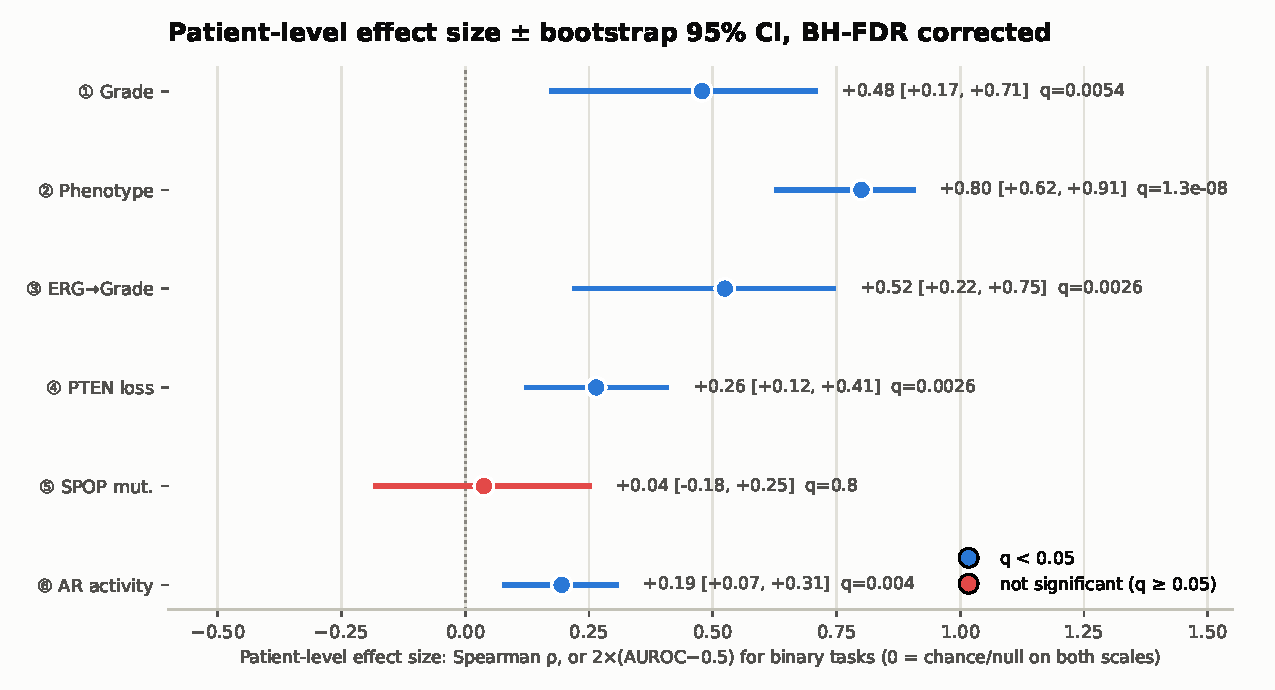
\includegraphics[width=0.75\textwidth]{figures/fig5_forest_plot.pdf}
\caption{Patient-level effect size $\pm$ bootstrap 95\% CI for the six initial frozen-pool
markers. AUROC-based markers are rescaled to $2\times(\mathrm{AUROC}-0.5)$ so that 0
represents chance on the same axis as Spearman $\rho$.}
\label{fig:forest}
\end{figure}

\begin{figure}[htbp]
\centering
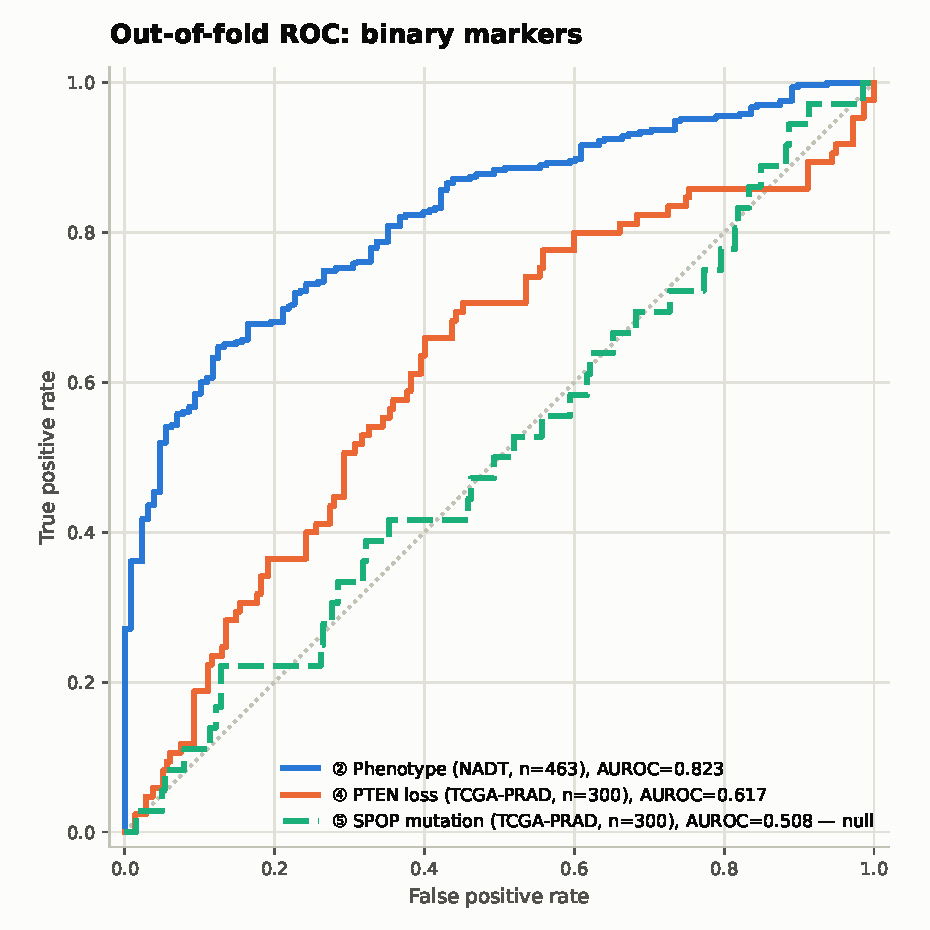
\includegraphics[width=0.85\textwidth]{figures/fig4_roc_curves.pdf}
\caption{Out-of-fold ROC curves for the three binary markers.}
\label{fig:roc}
\end{figure}

\subsection{Cross-encoder replication}

Every marker in the pool was re-evaluated with Virchow, a foundation model from a different
organization, architecture, and training corpus than CONCH. Agreement is close for markers 1,
2, and 4 in their primary
configurations. The completed grid shows that SPOP can cross chance in either direction under
both encoders and therefore does not support a clean cross-encoder null. Marker 3 (ERG) is
\emph{stronger} in Virchow. Marker 7 (recurrence) shows the largest divergence and is discussed
separately (Section~\ref{sec:res-marker7}): Gate A shows CONCH configuration means of
0.681--0.739 and Virchow means of 0.545--0.658, with Virchow improving at the shared
$1.76\,\mu$m/px scale. CONCH is higher in the current grid, while Virchow improves at the shared
$1.76\,\mu$m/px scale. Common-498 R2 preserves every scale, tile-budget, and shared-scale
encoder contrast direction without a raw-to-common null crossing. This closes the variable
source-retention check. The official-PFI C-index interval includes 0.5, so effect size and
transfer generalizability remain limited by endpoint, encoder, and scale; the completed
analysis does not establish robust independent prognostic value. By contrast, the nested confounder-audit increments for PTEN and AR
\emph{converge} rather than diverge across encoders (Section~\ref{sec:confounder-audits}) --
cross-encoder agreement can point the same way for a weak result as for a strong one, and both
are informative.

\begin{figure}[htbp]
\centering
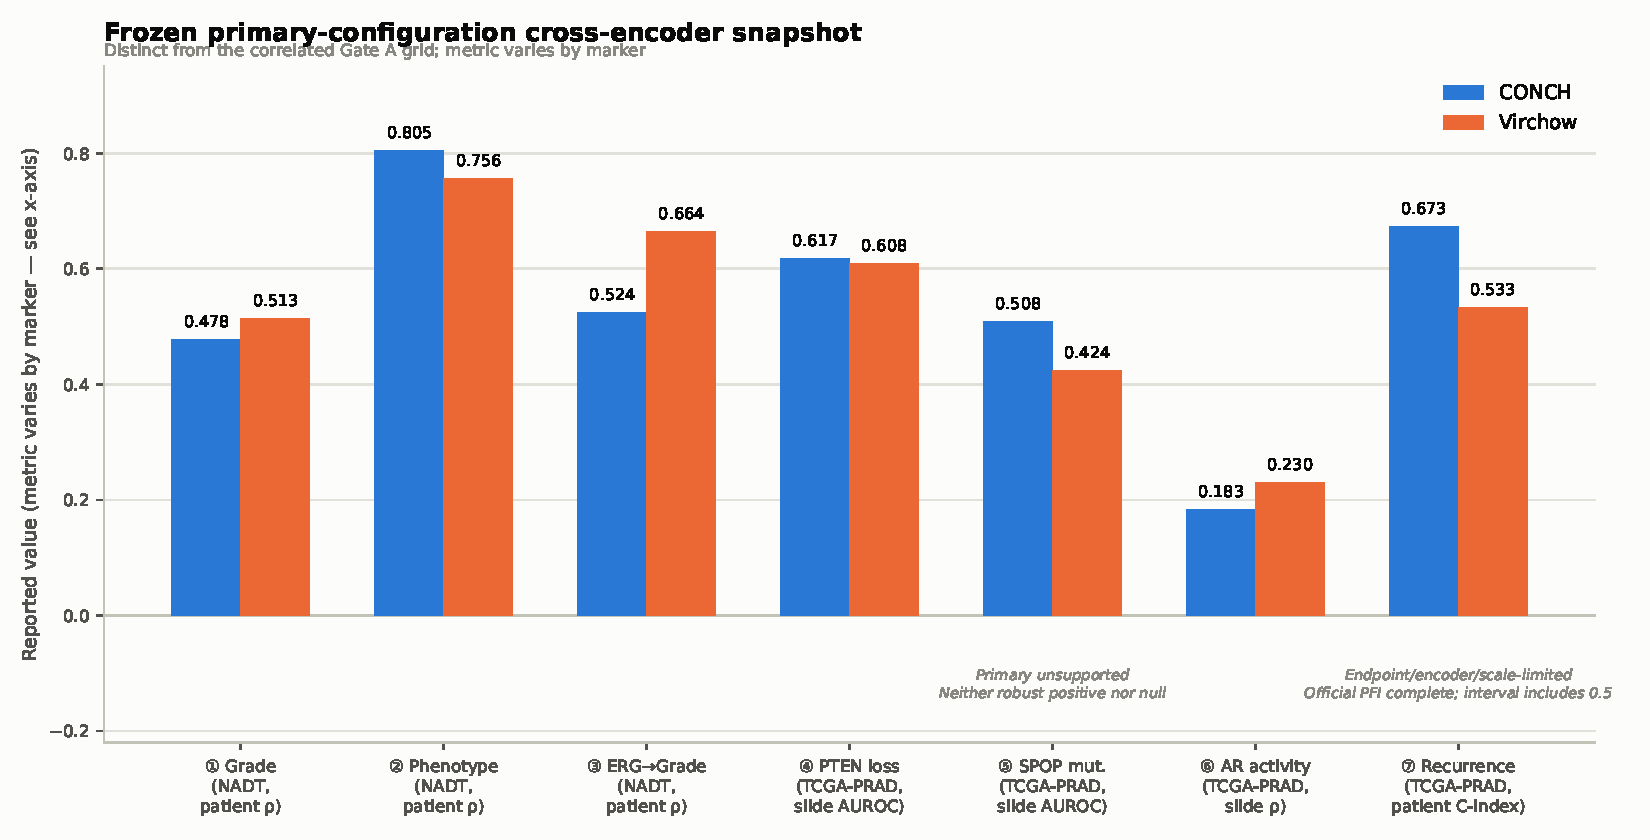
\includegraphics[width=0.92\textwidth]{figures/fig3_conch_vs_virchow.pdf}
\caption{This frozen primary-configuration snapshot compares CONCH/Virchow values for all seven
markers and is distinct from the correlated Gate A grid in Figure~\ref{fig:scale-heatmap}. Values use the metric named
for each marker and support only within-marker encoder comparison. The analysis units are
explicit: markers 1--3 and 7 are patient-level; markers 4--6 are slide-level. The SPOP primary
configuration is not supported; Gate A establishes neither a robust positive nor a robust null.
Marker 7 is endpoint/encoder/scale-limited; common-498 R2 and official-PFI R3 are complete,
and the official-PFI C-index interval includes 0.5.}
\label{fig:crossenc}
\end{figure}

\subsection{PRECISE: spatial face-validity and real-Gleason external validation}

Tile-level scoring against PRECISE's pixel-level expert annotations (Figure~\ref{fig:m1ext}a
scatter; annotation regions are small relative to standard tiling, requiring a
$150\,\mu$m window rather than the $\approx 394\,\mu$m used elsewhere to obtain any
qualifying benign-gland tiles) shows marker 1 in a clean monotonic order across tissue class:
benign gland (mean predicted grade 5.2) $\ll$ stroma (7.7) $<$ tumor (8.7) -- exactly the
expected pattern, since Gleason grading does not conceptually apply to benign tissue.

\textbf{Aggregation unit.} All PRECISE scoring is aggregated per imaging session (25 patients,
27 sessions total -- one patient contributes three sessions, all others one each; ``image'' in
this section always means one session, i.e.\ \texttt{sub-XX\_ses-YY}, not one patient). Averaged
per session and compared against real pathologist-assigned Gleason score, marker 1 achieves
Spearman $\rho=+0.87$ ($p=7.6\times10^{-6}$, $n=17$ sessions), zero-shot, on a cohort never used
in any training step. As a robustness check against over-counting patients with multiple
sessions: all 17 sessions in this specific real-Gleason comparison happen to come from 17
distinct patients (the one multi-session patient's other two sessions either lacked a
comparable Gleason label or no qualifying tumor tile), so the session-level and patient-level
aggregations of this particular result are numerically identical ($\rho=+0.87$ either way) --
the correlation is not an artifact of any patient being over-represented. Marker 2 (phenotype)
preserves the correct ordinal direction (tumor $>$ benign $>$ stroma by median tumor-probability)
but saturates near ceiling at this fine spatial scale, a granularity mismatch with NADT's
coarser whole-slide training signal that we report as an honest limitation rather than a
further positive result.

\subsection{QWK and comparison to literature}

Figure~\ref{fig:m1ext}b converts marker 1's continuous predictions to quadratic weighted kappa
(QWK) for direct comparison with literature figures reported in that unit. Zero-shot QWK
($0.26$--$0.39$) is well below fully supervised PANDA-challenge-winner performance ($\approx
0.86$), an expected gap given this study evaluates a frozen general-purpose embedding with a
linear probe and zero retraining against purpose-built, massively supervised models -- a gap
consistent with, not contradicting, this study's positioning as a reproducibility and
transportability audit rather than a grading-accuracy benchmark. PRECISE's real-Gleason QWK
($0.788$) approaches the supervised benchmark but is based on only 17 images and should not be
over-interpreted as a comparable-scale result.

\begin{figure}[htbp]
\centering
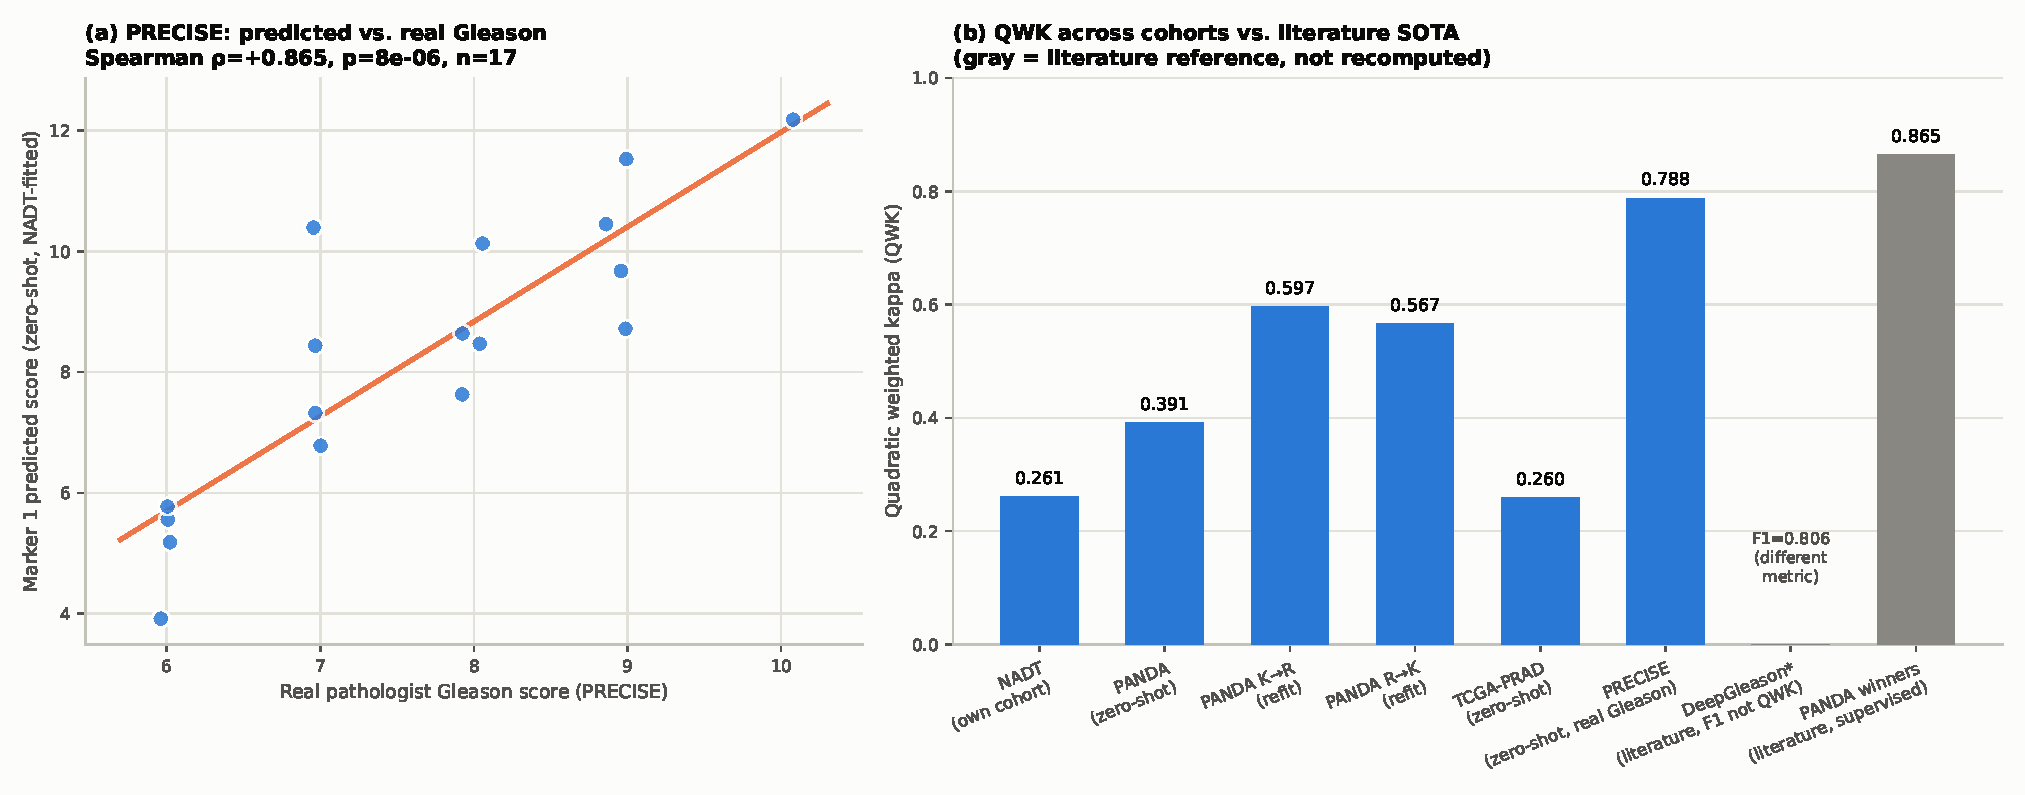
\includegraphics[width=0.98\textwidth]{figures/fig2_marker1_external.pdf}
\caption{(a) Marker 1 predicted vs.\ real pathologist Gleason score on PRECISE. (b) QWK across
all evaluated cohorts and two literature reference points (gray).}
\label{fig:m1ext}
\end{figure}
